\section{Experiments}

We performed the following experiments using our prototype to validate the protocol.

\subsection{Cover Traffic}

\begin{figure}
\begin{center}
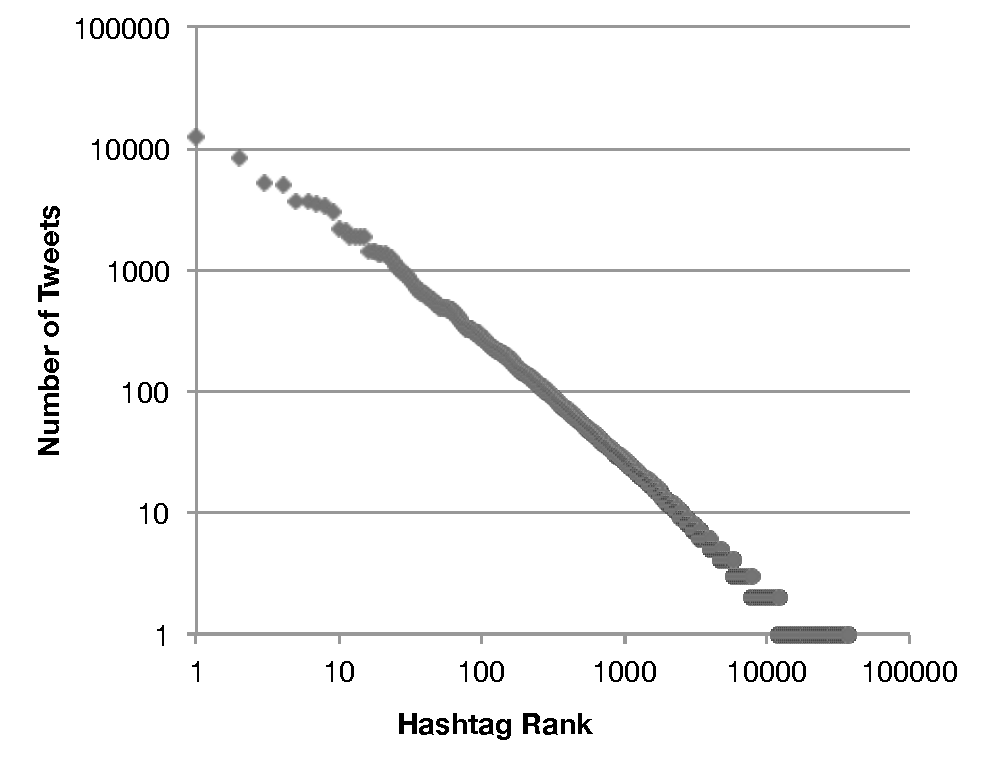
\includegraphics[scale=.4, viewport= 0cm 0cm 20.6cm 12.9cm]{hash-tag-dist.pdf}
\caption{2009 Twitter Hash Tag distribution on a log-log scale.
\label{fig:hash-dist}
}
\end{center}
\end{figure}

The power log scale shows us that there is a large spectrum of subscriber anonymity that can be taken advantage of. 

\hl{--How long a short tag should be? Should we break down log-log scale further, or simply examine average tag length?}

\hl{size 8 seems to eliminate most collisions, allows for exact look up should you choose it.}

\subsection{Collider}

In order to explore the feasibility of steering a particular Plain Tag to collide with an existing Short Tag, we built a collider tool. The tool takes in a Short Tag substring, \textit{T}, a prefix string, \textit{S}, a suffix length, \textit{L}, an alphabet 
\textit{A}. The collider finds all concatenations of \textit{S} and strings of length \textit{L} from \textit{A*} such that the truncated hash of the resultant string matches \textit{T}.

The search space, then, is of size $|A|^L$. If we wanted to match byte strings, $|A| = 256$, however, we decided to restrict the alphabet to alphanumeric characters, yielding $|A| = 62$. Additionally, the search space can be explored in parallel, giving the Collider executing on a system with \textit{P} processing units, a runtime of $O(\frac{62^L}{P})$. \hl{(this is incredibly parallel so easier to bruteforce)}

\begin{figure}
\begin{center}
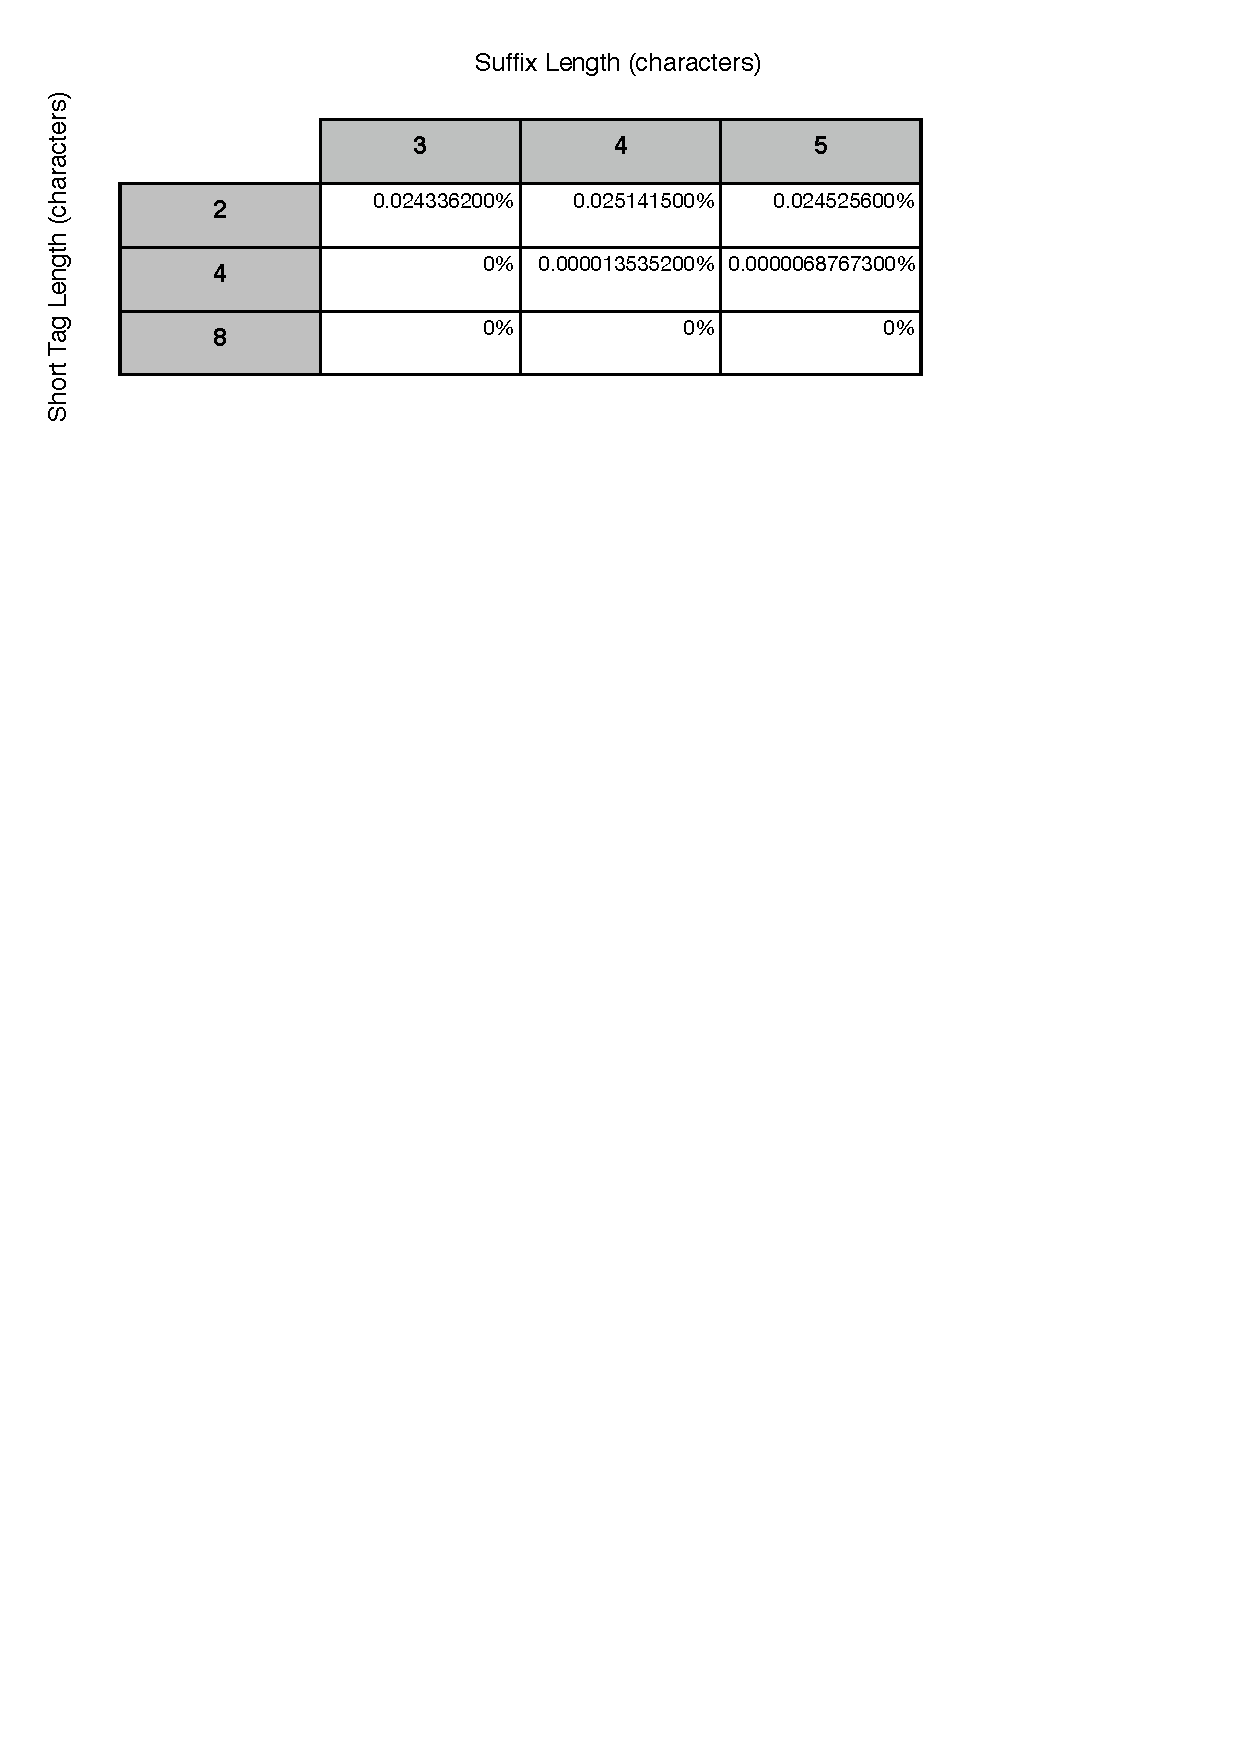
\includegraphics[scale=.5, viewport= 0cm 0cm 16.5cm 7.5cm]{collider-hits.pdf}
\caption{Percent of search space that returned hits for an entered Short Tag, with a Prefix of `rice', and given Suffix Length.
\label{fig:collider-hits}
}
\end{center}
\end{figure}

\begin{figure}
\begin{center}
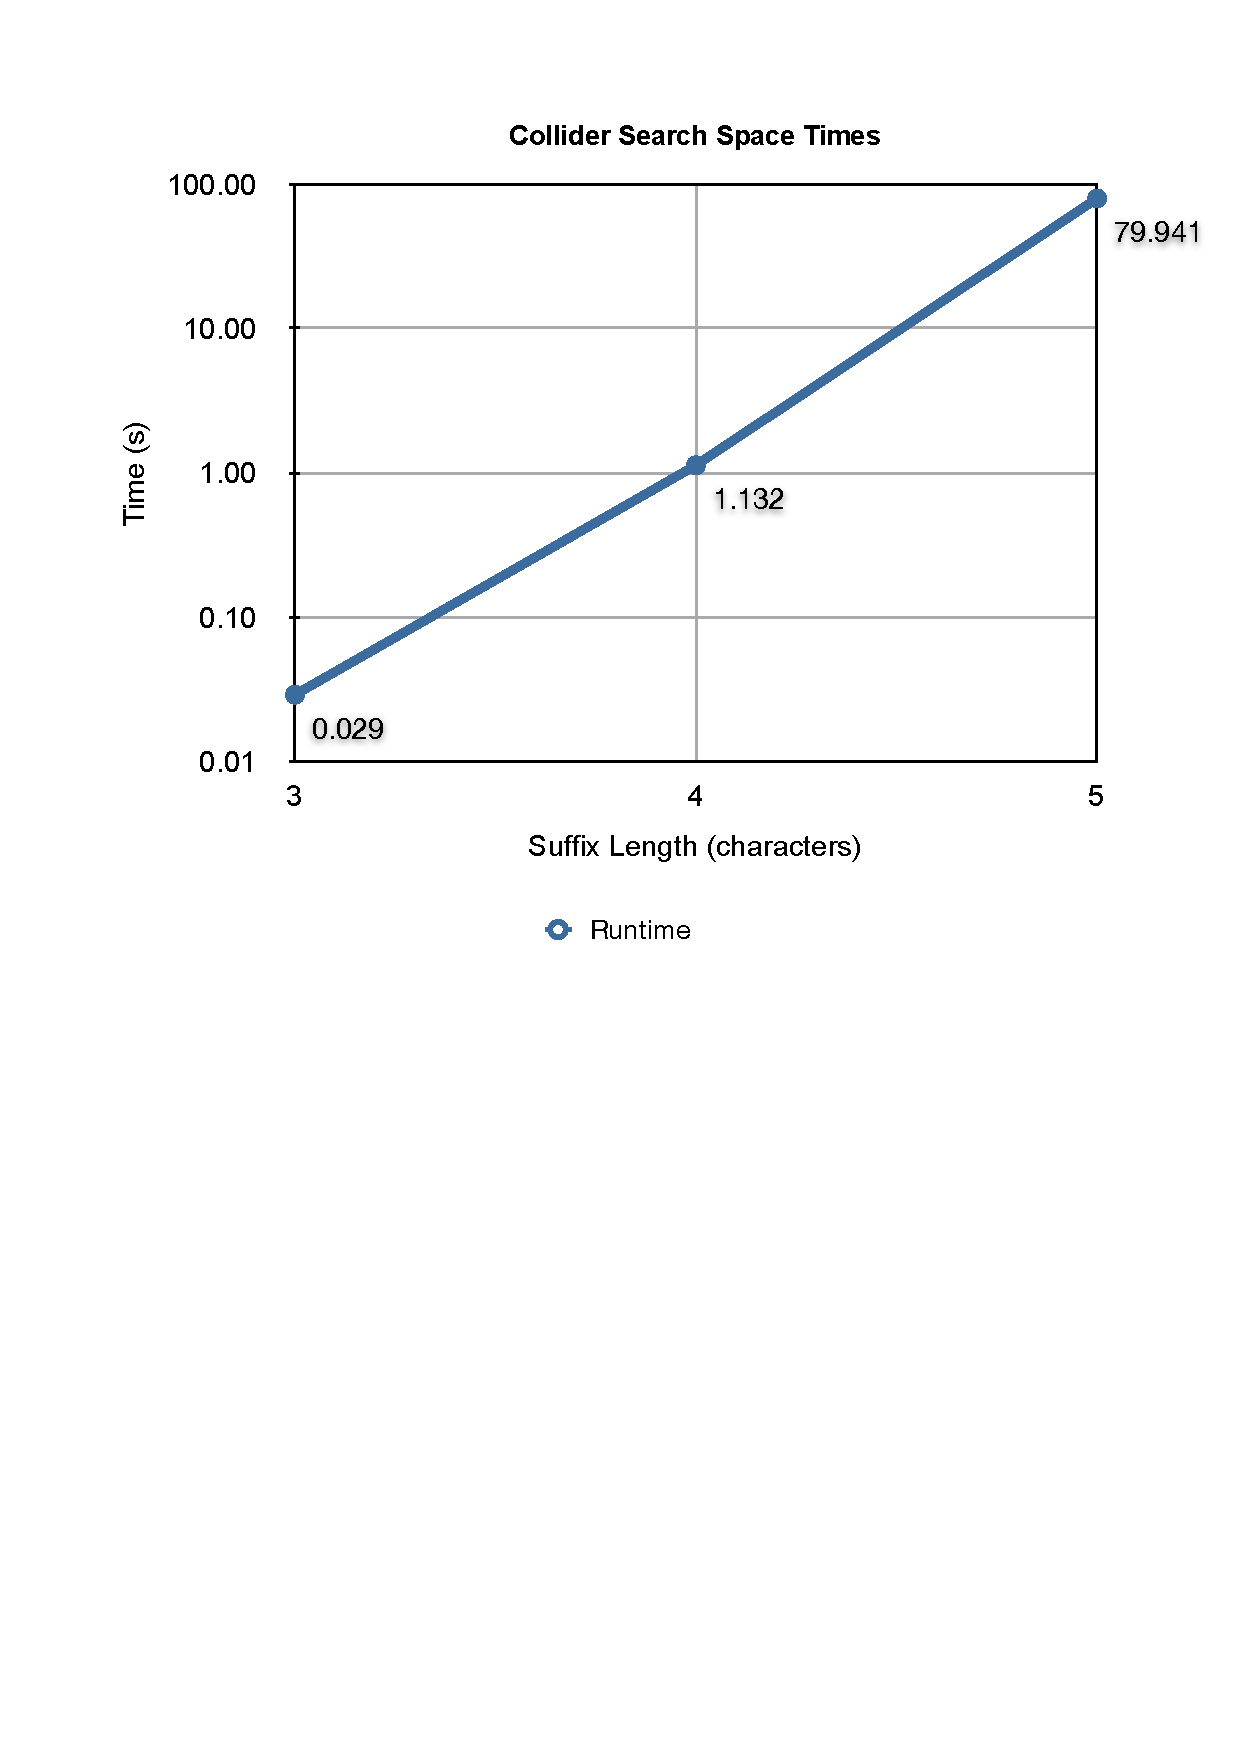
\includegraphics[scale=.5, viewport= 1cm 0.5cm 19.5cm 15.5cm]{collider-times.pdf}
\caption{Runtime for the Collider to search the exploration spaces of sizes $62^3$, $62^4$, $62^5$ on dual quad-core Intel i5 processors.
\label{fig:collider-times}
}
\end{center}
\end{figure}


As expected, the runtime in Figure \ref{fig:collider-times} scales exponentially with \textit{L}. 


\hl{
- what that tells us about design parameters of solution \\
- Then we can conclude that we need this number of bits, etc\\
- Wrap up all experiments into What can our system do\\
- Easy to collide or not to collide (Tune cover traffic)\\
}

\subsection{Performance}

In this experiment we wanted to see how well the encryption engine performed. In March 2011, Twitter stated that the site receives 140 million tweets per day or 1620 tweets per second on average (http://blog.twitter.com/2011/03/numbers.html). They also said that the maximum tweets per second ever was 6939. These numbers act as rough upper bounds to the number of Hoots per second the system would need to keep up with. In all likelihood, the number of encrypted messages posted would be drastically smaller than regular messages.

The benchmarks in Table \ref{tab:hps} were run on a 1.86GHz Intel Core 2 Duo, 4GB Ram, Macbook Air using Base64 encoding.


\begin{table}
\caption{Average Hoots Per Second for Encryption and Decryption
\label{tab:hps}
}
\begin{center}
    \begin{tabular}{ l  l }
	\hline
	Action & Average Hoots per second \\ \hline
	Encryption & 3614.531 \\
	Decryption & 15587.328 \\ \hline
    \end{tabular}
\end{center}
\end{table}

Given these numbers, a Twitter server could easily encrypt the entire Twitter feed as the messages were posted. To handle peak usage like the 6939 tweets per second Twitter observed, many optimizations could be made, the simplest being to add a couple computers to help with the load. Our experiment shows that the Hoot protocol does not have significant overhead during encryption or decryption, so it can be adopted with little engineering effort.

It is interesting to note that the decryption rate is important to a client, since a client will be searching tweets trying to identify and decrypt potential Hoots. A client may not trust Twitter to do the decryption since that involves sharing the Plain Tag with Twitter, so a client would decrypt the message on their machine. Almost every client will not have a datacenter of computers for decryption, but our  process can decrypt Hoots almost five times faster than it encrypts them. A client, even with limited computing power, can easily keep up with the Twitter feed.